\documentclass[conference]{IEEEtran}

\IEEEoverridecommandlockouts
% The preceding line is only needed to identify funding in the first footnote. If that is unneeded, please comment it out.
\usepackage{cite}
\usepackage{amsmath,amssymb,amsfonts}
\usepackage{algpseudocode}
\usepackage{algorithm2e}
\usepackage{graphicx}
\usepackage{textcomp}
\usepackage{xcolor}
\usepackage{hyperref}
\usepackage{comment}

\def\BibTeX{{\rm B\kern-.05em{\sc i\kern-.025em b}\kern-.08em
    T\kern-.1667em\lower.7ex\hbox{E}\kern-.125emX}}

\begin{document}

\input{Document/Titlepage}

\begin{comment}
\begin{abstract}
This document is a model and instructions for \LaTeX.
This and the IEEEtran.cls file define the components of your paper [title, text, heads, etc.]. *CRITICAL: Do Not Use Symbols, Special Characters, Footnotes, 
or Math in Paper Title or Abstract.
\end{abstract}

\begin{IEEEkeywords}
component, formatting, style, styling, insert
\end{IEEEkeywords}
\end{comment}


\section{INTRODUCCION}
Las simulaciones de colisiones galácticas son importantes debido a que permiten predecir de forma teórica el comportamiento de dos galaxias en cercanía y determinar las probabilidades de colisiones entre sí a futuro.
El modelado y simulaciones de galaxias y cuerpos celestes presenta retos numéricos y computacionales, esto es causado a la gran cantidad de cuerpos que se tiene que usar y las diferentes interacciones que estos manejan. Una de las prioridades de las simulaciones se aproximen lo mejor posible a un escenario realista y que el tiempo de ejecución no sea tan alto.

\section{OBJETIVOS}
\IEEEPARstart {} En el presente proyecto se plantearon los siguientes objetivos:
\begin{itemize}
    \item Diseño del PRAM del problema de N-cuerpos.
    \item Ejecutar pruebas con diferentes cantidad de cuerpos y procesadores.
    \item Medir el tiempo de ejecución, cálculo de la fuerza, tiempo de comunicación entre procesos y los GFlops.
    \item Realizar comparaciones de los resultados obtenidos del \textit{speedup} y eficiencia.
    \item Determinar la escalabilidad del algoritmo.
\end{itemize}

\section{MARCO TEÓRICO}
En el desarrollo e implementación del software se utilizaron dos conceptos para determinar cuan escalable son los códigos, estos son: Escalamiento fuerte, escalamiento débil , eficiencia de escalamiento fuerte, eficiencia de escalamiento débil, curva de isoeficiencia.



\subsection{ESCALAMIENTO FUERTE (Strong Scaling) }
En el caso de los resultados provistos, el tamaño del problema permanece fijo pero aumenta el número de elementos de procesamiento. Esto se usa como justificación para los programas que tardan mucho en ejecutarse. En una escala fuerte, se considera que un programa escala linealmente si el speed-up es igual al número de elementos de procesamiento utilizados [3].

\begin{figure}[h]
    \centering
    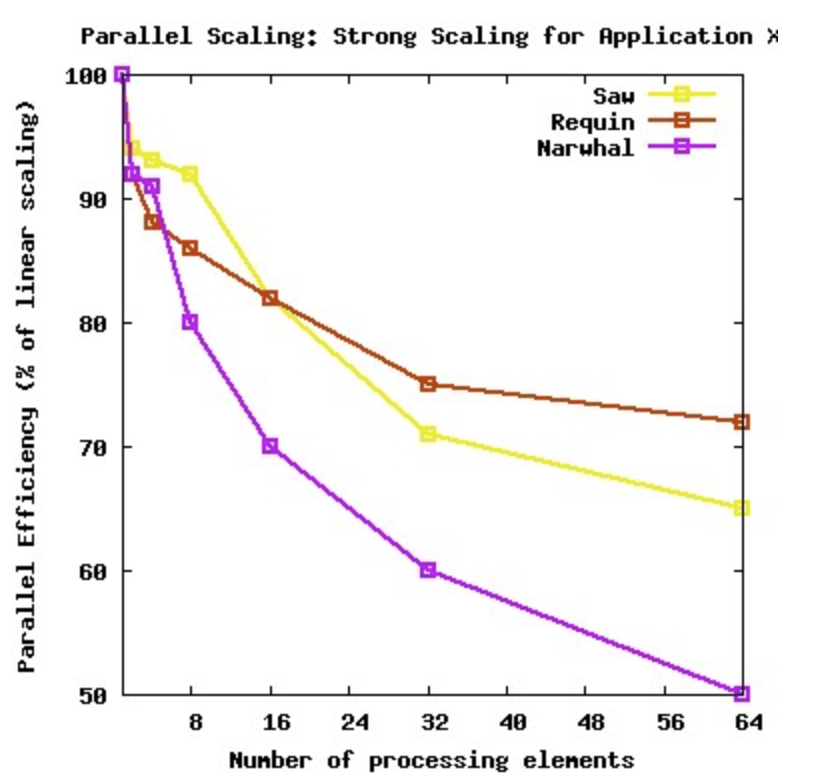
\includegraphics[width =6.4cm]{Images/bibliografia.png}
    \caption{Escalado fuerte: escalamiento fuerte para la aplicación x[4].}
    \label{fig:my_label}
\end{figure}

\subsection{EFICIENCIA DE ESCALAMIENTO FUERTE\\}
 Ruby Lee en 1980 definió varios parámetros para evaluar el cálculo paralelo. A continuación se muestra la definición de dichos algunos  parámetros.\\

Sea O(n) el número total de operaciones elementales realizadas
por un sistema con n elementos de proceso, y T(n) el tiempo de ejecución en pasos unitarios de tiempo. En general, T(n) < O(n) si los n procesadores realizan más de una operación por unidad de tiempo, donde $ n \geq 2 $. Supongamos que T(1) = O(1) en un sistema mono-procesador, lo cual supone que IPC = 1 (IPC= Instrucciones Por Ciclo). El factor de mejora del rendimiento (speed-up, aceleración o rapidez) se define como:
\begin{equation}
  S_{n}= \frac{T_{1}}{T_{n}}
\end{equation}
La eficiencia del sistema para un sistema con n procesadores se define como:
\begin{equation}
    E_{n}= \frac{S_{n}}{n} = \frac{T_{1}}{p*T_{n}}
\end{equation}



\section{METODOLOGÍA}
En primer lugar para realizar nuestro cálculos de manera teórica diseñamos el siguiente PRAM al cual se le añadió el costo de comunicación.

\RestyleAlgo{ruled}

%% This is needed if you want to add comments in
%% your algorithm with \Comment
\SetKwComment{Comment}{/* }{ */}
%%% this is from the switches further in the package
\SetKwInput{KwIn}{Input}%
\SetKwInput{KwOut}{Salida}%
\SetKwInput{KwData}{Entrada}%
\SetKwInput{KwResult}{Result}%

\begin{algorithm}[hbt!]
\caption{PRAM N-cuerpos}\label{alg:two}
\KwData{Todos las partículas con masa,posición,velocidad,aceleración}
\KwOut{Un dataset con el resultado de las interacciones con los diferentes cuerpos.}
\For{$i\gets1$ \KwTo $N$}{
    \zeta_{i} $\gets$ read(datos)
}
$ broadcast(N)$
$AllScatter(... \zeta_{\frac{n}{p}})$\\

\While{$i < N$}{ \textbf{pardo}\\
    $my_{x}:= \zeta.rx$\;
    $my_{y}:= \zeta.ry$\;
    $my_{z}:= \zeta.rz$\;
    \While{$j < N$}{
        \If{$ i \neq j $}{
            $d_{x} := \zeta_{x_{j}} - my_{x}$\;
            $d_{y} := \zeta_{y_{j}} - my_{y}$\;
            $d_{z} := \zeta_{z_{j}} - my_{z}$\;
            $\textbf{send(i)|receive(j)}$\;
            $a_{x} := \frac{G*my_{i}my_{j}}{d_{x}^2} $\;
            $a_{y} := \frac{G*my_{i}my_{j} }{d_{y}^2} $\;
            $a_{z} := \frac{G*my_{i}my_{j}}{d_{z}^2} $\;
        }  
    }
    \While{$l < N$}{ \textbf{pardo}\\
        $\zeta.vx{i}:=a_{x} \triangle t s$\;
        $\zeta.vy{i}:=a_{y} \triangle t s$\;
        $\zeta.vz{i}:=a_{z} \triangle t s$\;
        $\zeta.rx{i}:=v_{z} \triangle t s$\;
        $\zeta.ry{i}:=v_{z} \triangle t s$\;
        $\zeta.rz{i}:=v_{z} \triangle t s$\;
    }
    \While{$k < N$}{
        $AllGather(... \zeta_{\frac{n}{p}}) $
    }
}

\end{algorithm}

\newpage 
Para el desarrollo del análisis se utilizo el generador N-cuerpos gen-plum como primer componente para obtener información de nuestra utilidad, dicho generador nos brindo un conjunto de datos que variaba según la modificación del parámetro N o cantidad de partículas. Luego utilizamos dicha información para ejecutar el programa cpu-4th que nos brindaba multiples estadísticas en ellas que usaríamos más adelante como: speed,tiempo de comunicación, tiempo total de ejecución, tiempo en el cálculo de la fuerza entre otros.
Una vez terminada la ejecución según la cantidad de cuerpos y cantidad de procesadores empleados, derivamos las múltiples salidas a archivos .txt con nombre del numero de partículas empleadas seguida del número de procesadores empleados en esa prueba. Después, se utiliza cada una de estas salidas como insumo para un programa .sh para generar archivos .txt pero esta vez con la información relevante obtenida a través de lenguaje \textit{bash} el cual realiza una consulta al usuario de que información quisiera obtener y capturarla. \\

\begin{figure}[!ht]
    \centering
    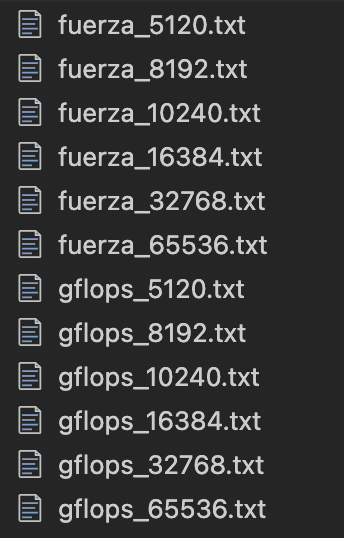
\includegraphics[width =2.5cm]{Images/script.png}
    \caption{Documentos retornados luego de ejecutar el script}
    \label{fig:my_label}
\end{figure}

Luego creamos un archivo .gnu y empleamos gnuplot a partir de la información devuelta por el script para graficar las diferentes variables que desarrollaremos en nuestro análisis. Finalmente se desarrollo un software en lenguaje python para poder obtener las estadísticas y datos relevantes de manera mucho más interactiva. \\

Como último detalle, utilizamos Khipu, supercomputador de \href{https://web.khipu.utec.edu.pe}{\textt{UTEC}}. Específicamente el procesador \href{https://web.khipu.utec.edu.pe/}{\textt{Intel(R)}} Xeon(R) Gold 6230 CPU @ 2.10GHz.


\section{RESULTADOS}
Ejecutamos el programa principal modificando el tamaño de los datos, $N = $ {5k, 8k, 10k, 16k, 32k, 64k} y del archivo de salida que obtenemos, se extrae los datos que necesitamos.

\begin{figure}[!ht]
    \centering
    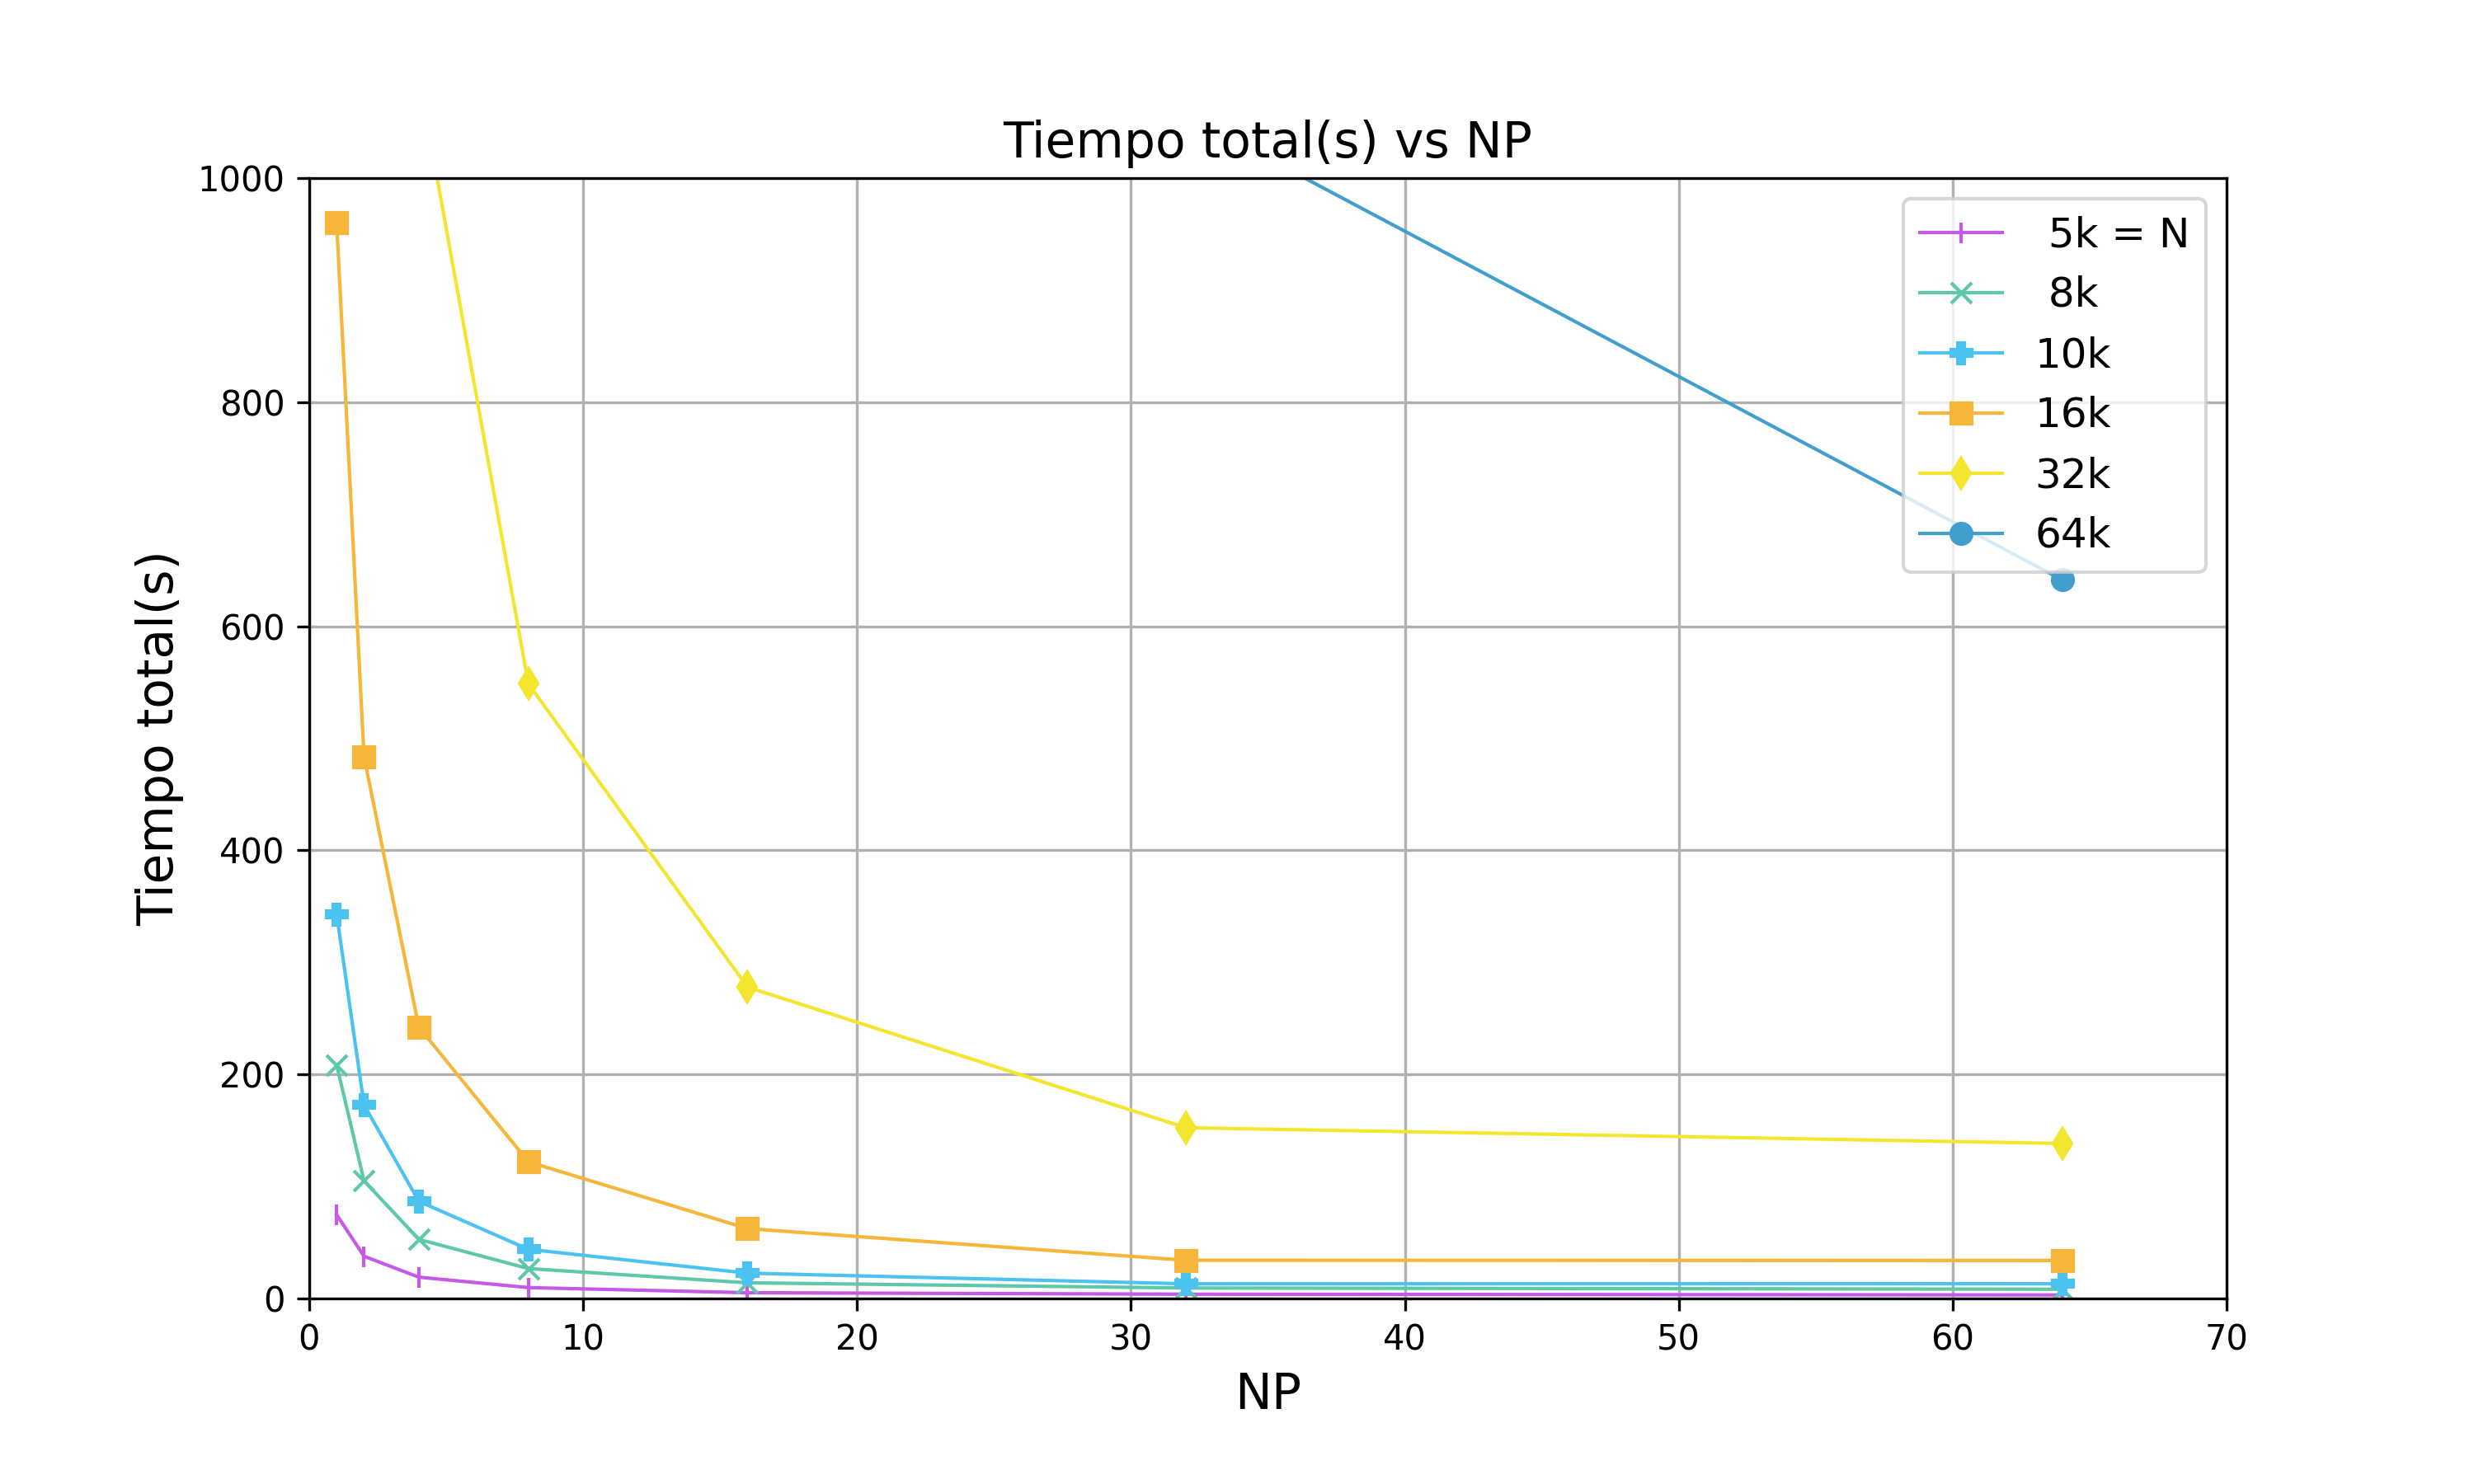
\includegraphics[width =7.5cm]{Images/Tiempo total(s) vs NP.png}
    \caption{Tiempo total de ejecución (s) vs NP}
    \label{fig:my_label}
\end{figure}

\begin{figure}[!ht]
    \centering
    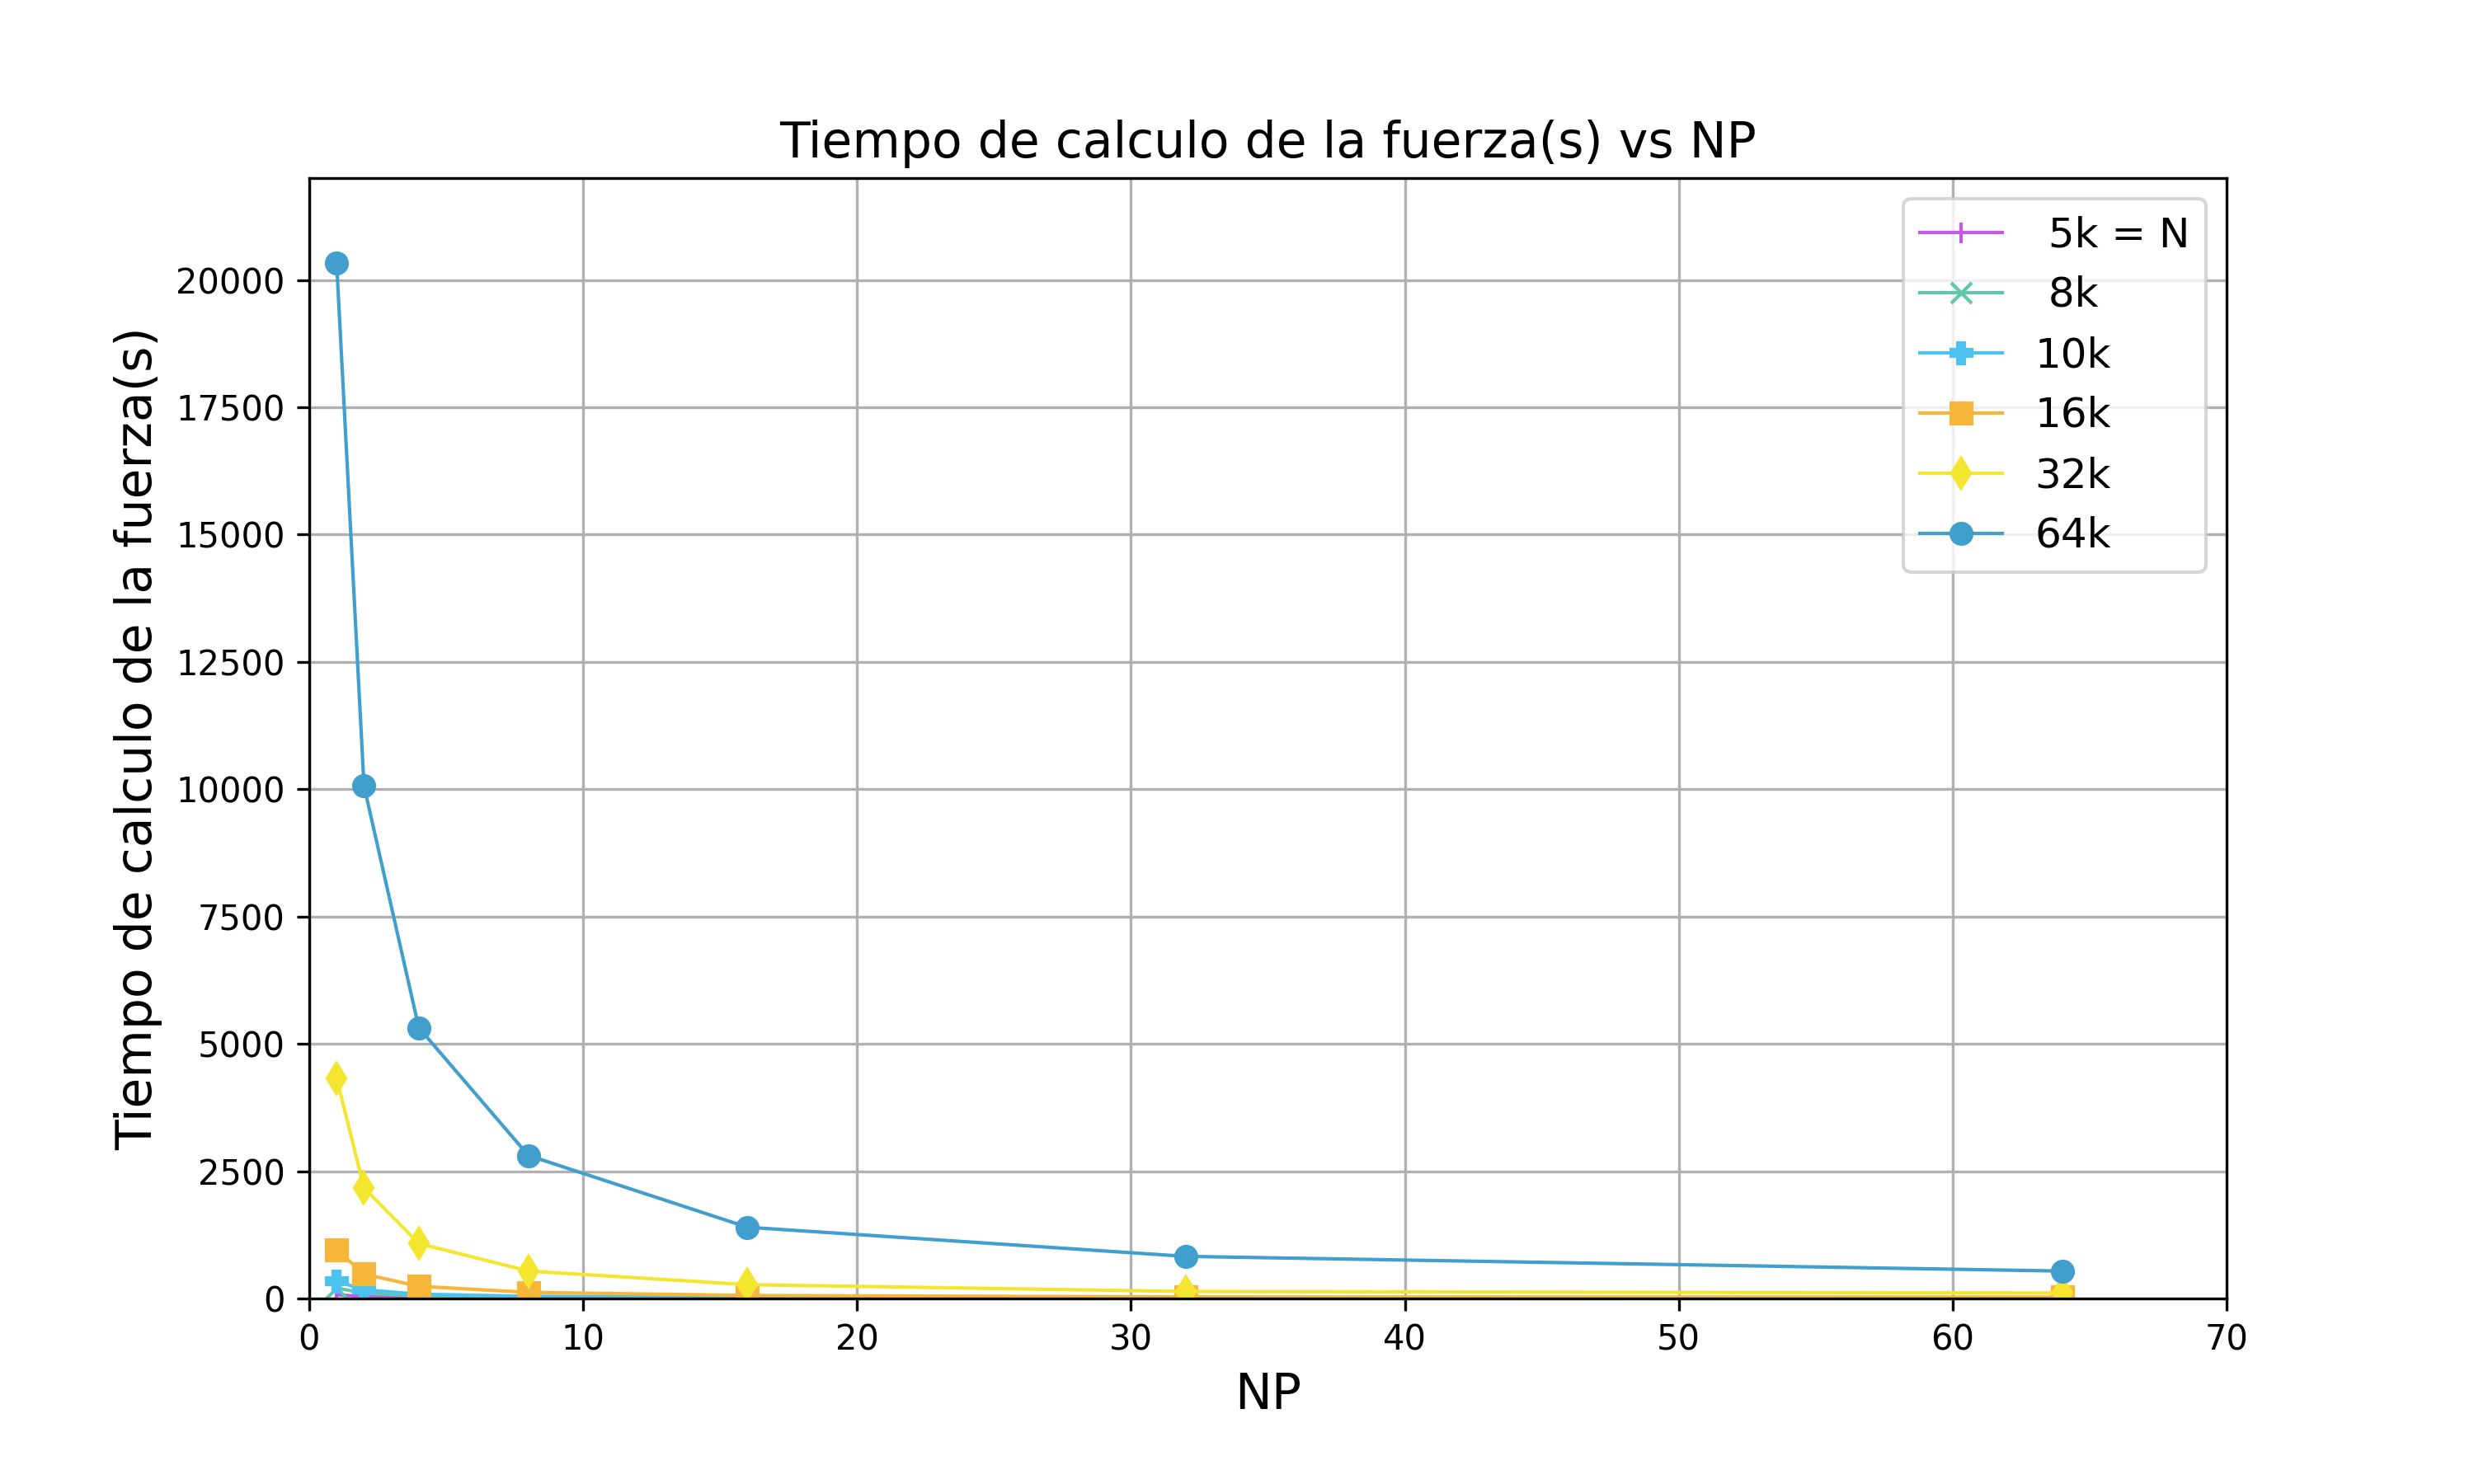
\includegraphics[width =7.5cm]{Images/Tiempo de calculo de la fuerza(s) vs NP.png}
    \caption{Tiempo del cálculo de la función calc\_force (s) vs NP}
    \label{fig:my_label}
\end{figure}

\begin{figure}[!ht]
    \centering
    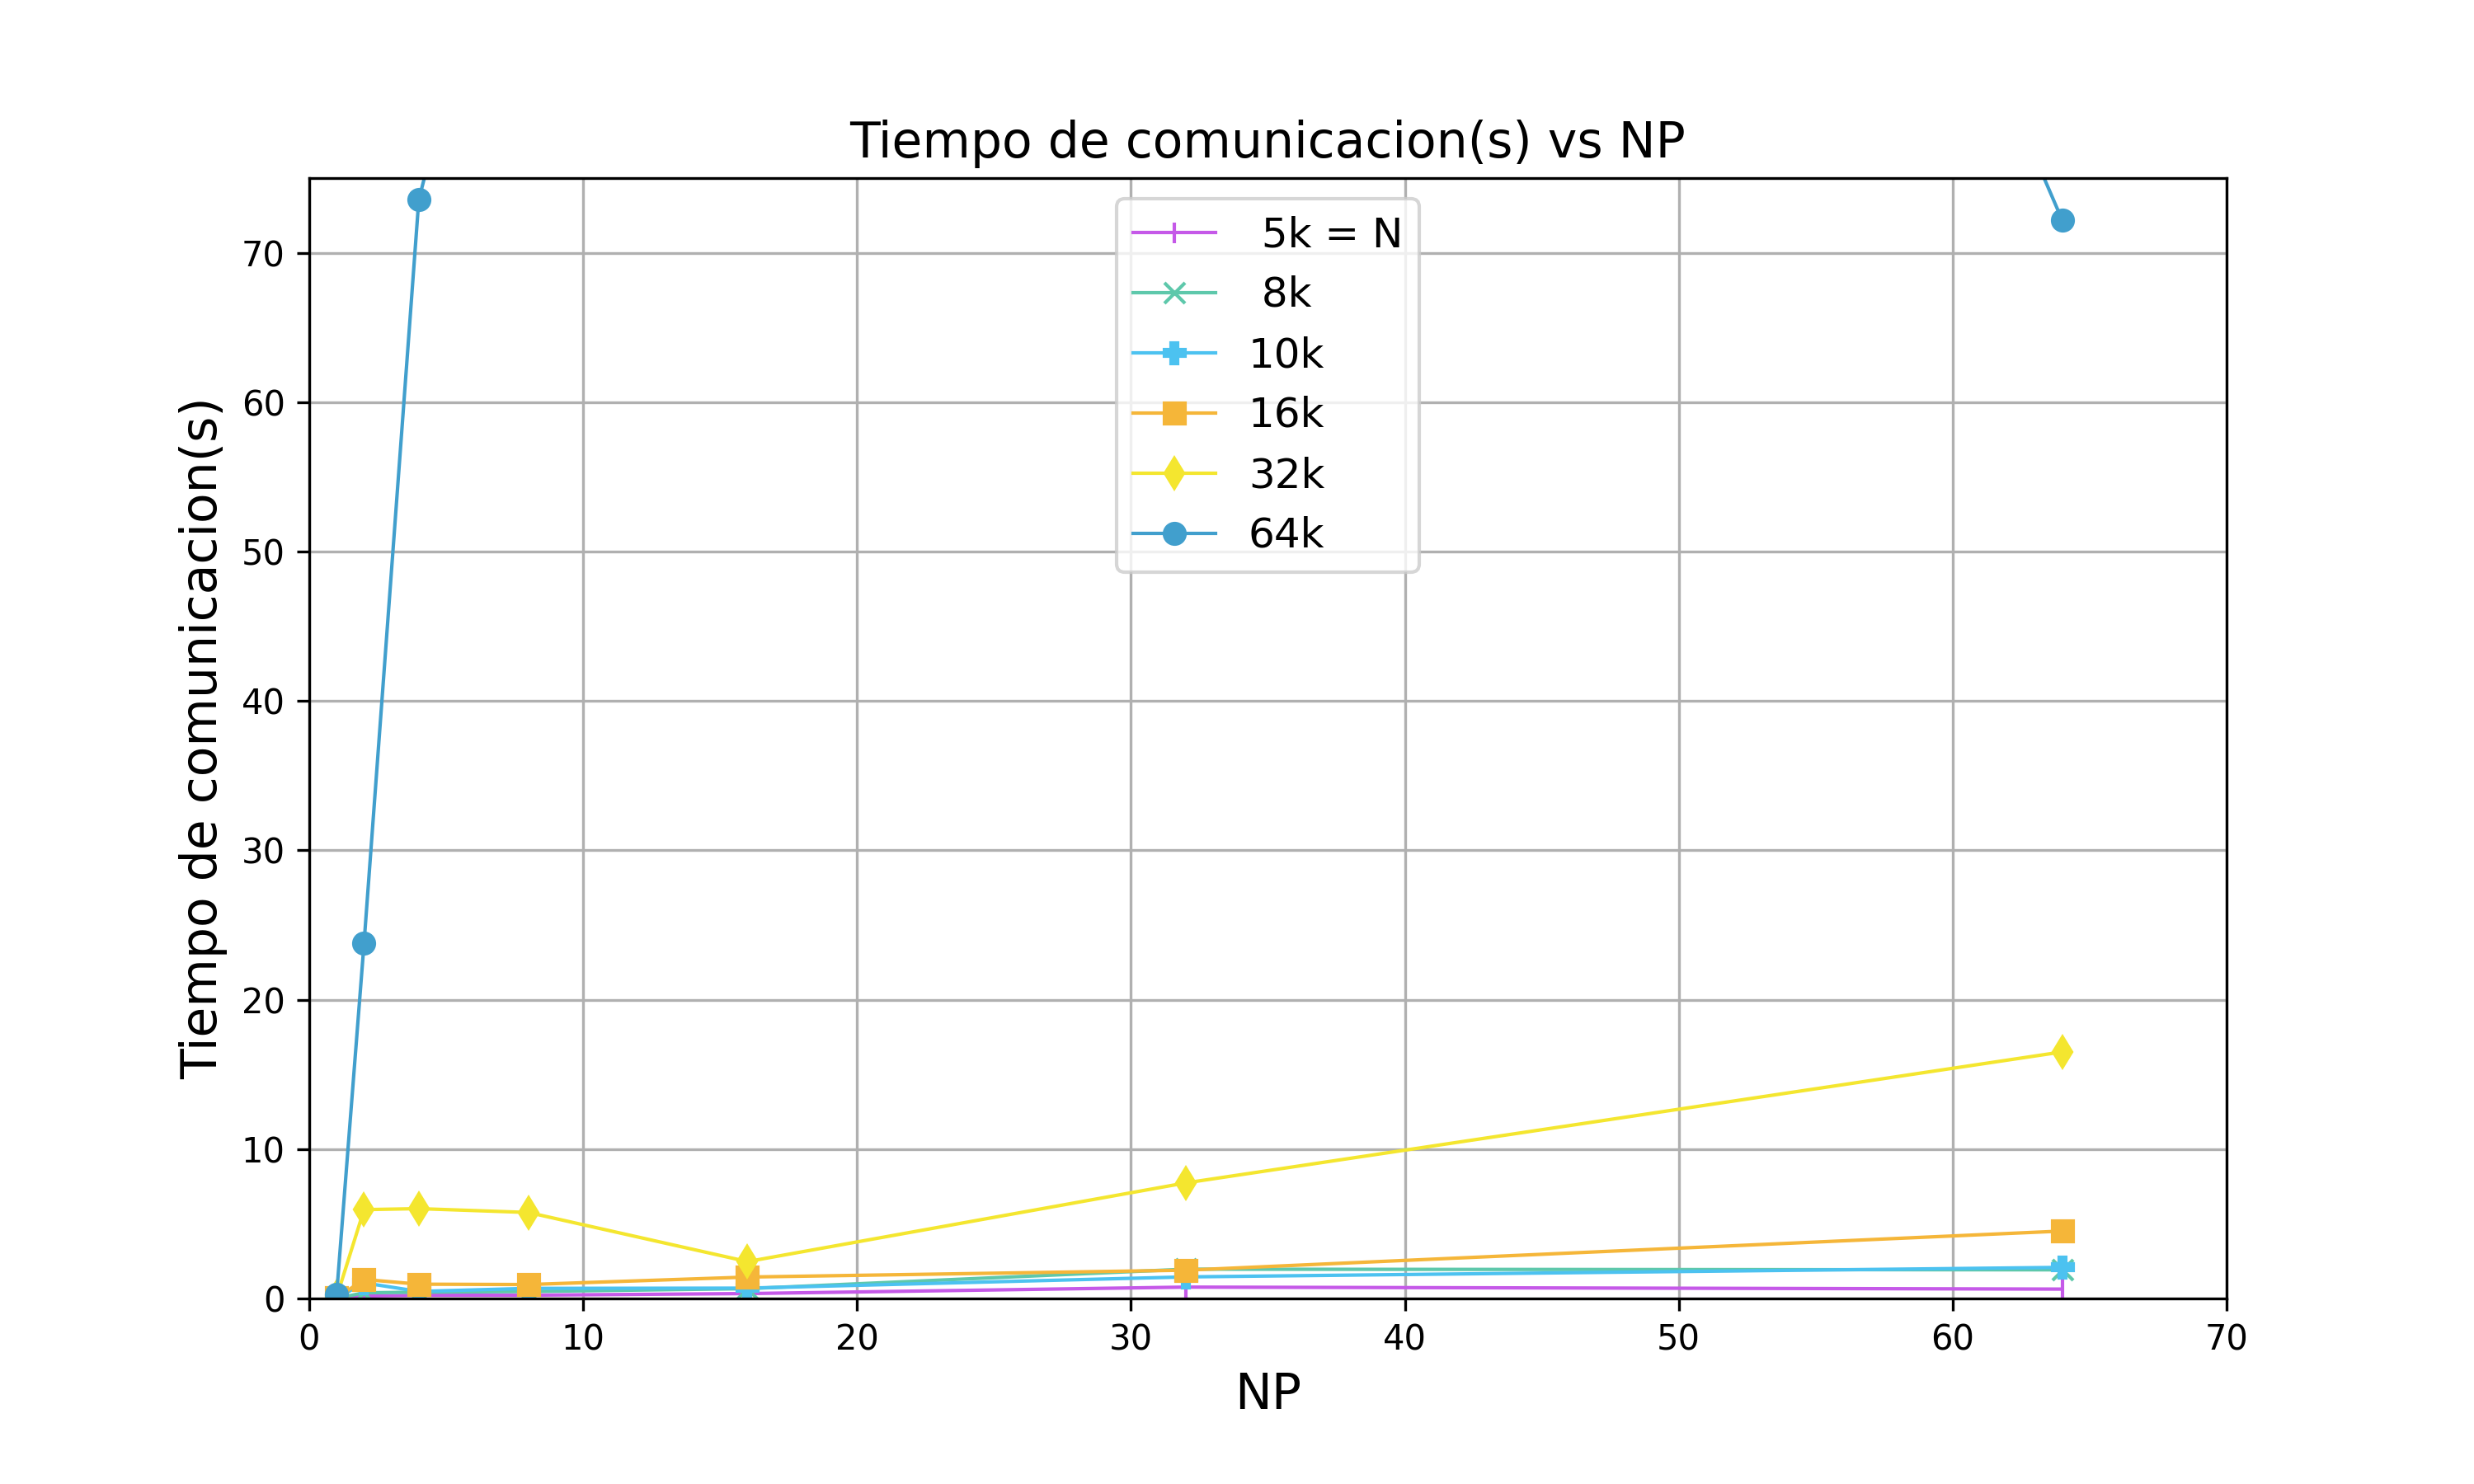
\includegraphics[width =7.5cm]{Images/Tiempo de comunicacion(s) vs NP.png}
    \caption{Tiempo de Comunicación (s) vs NP}
    \label{fig:my_label}
\end{figure}

\begin{figure}[!ht]
    \centering
    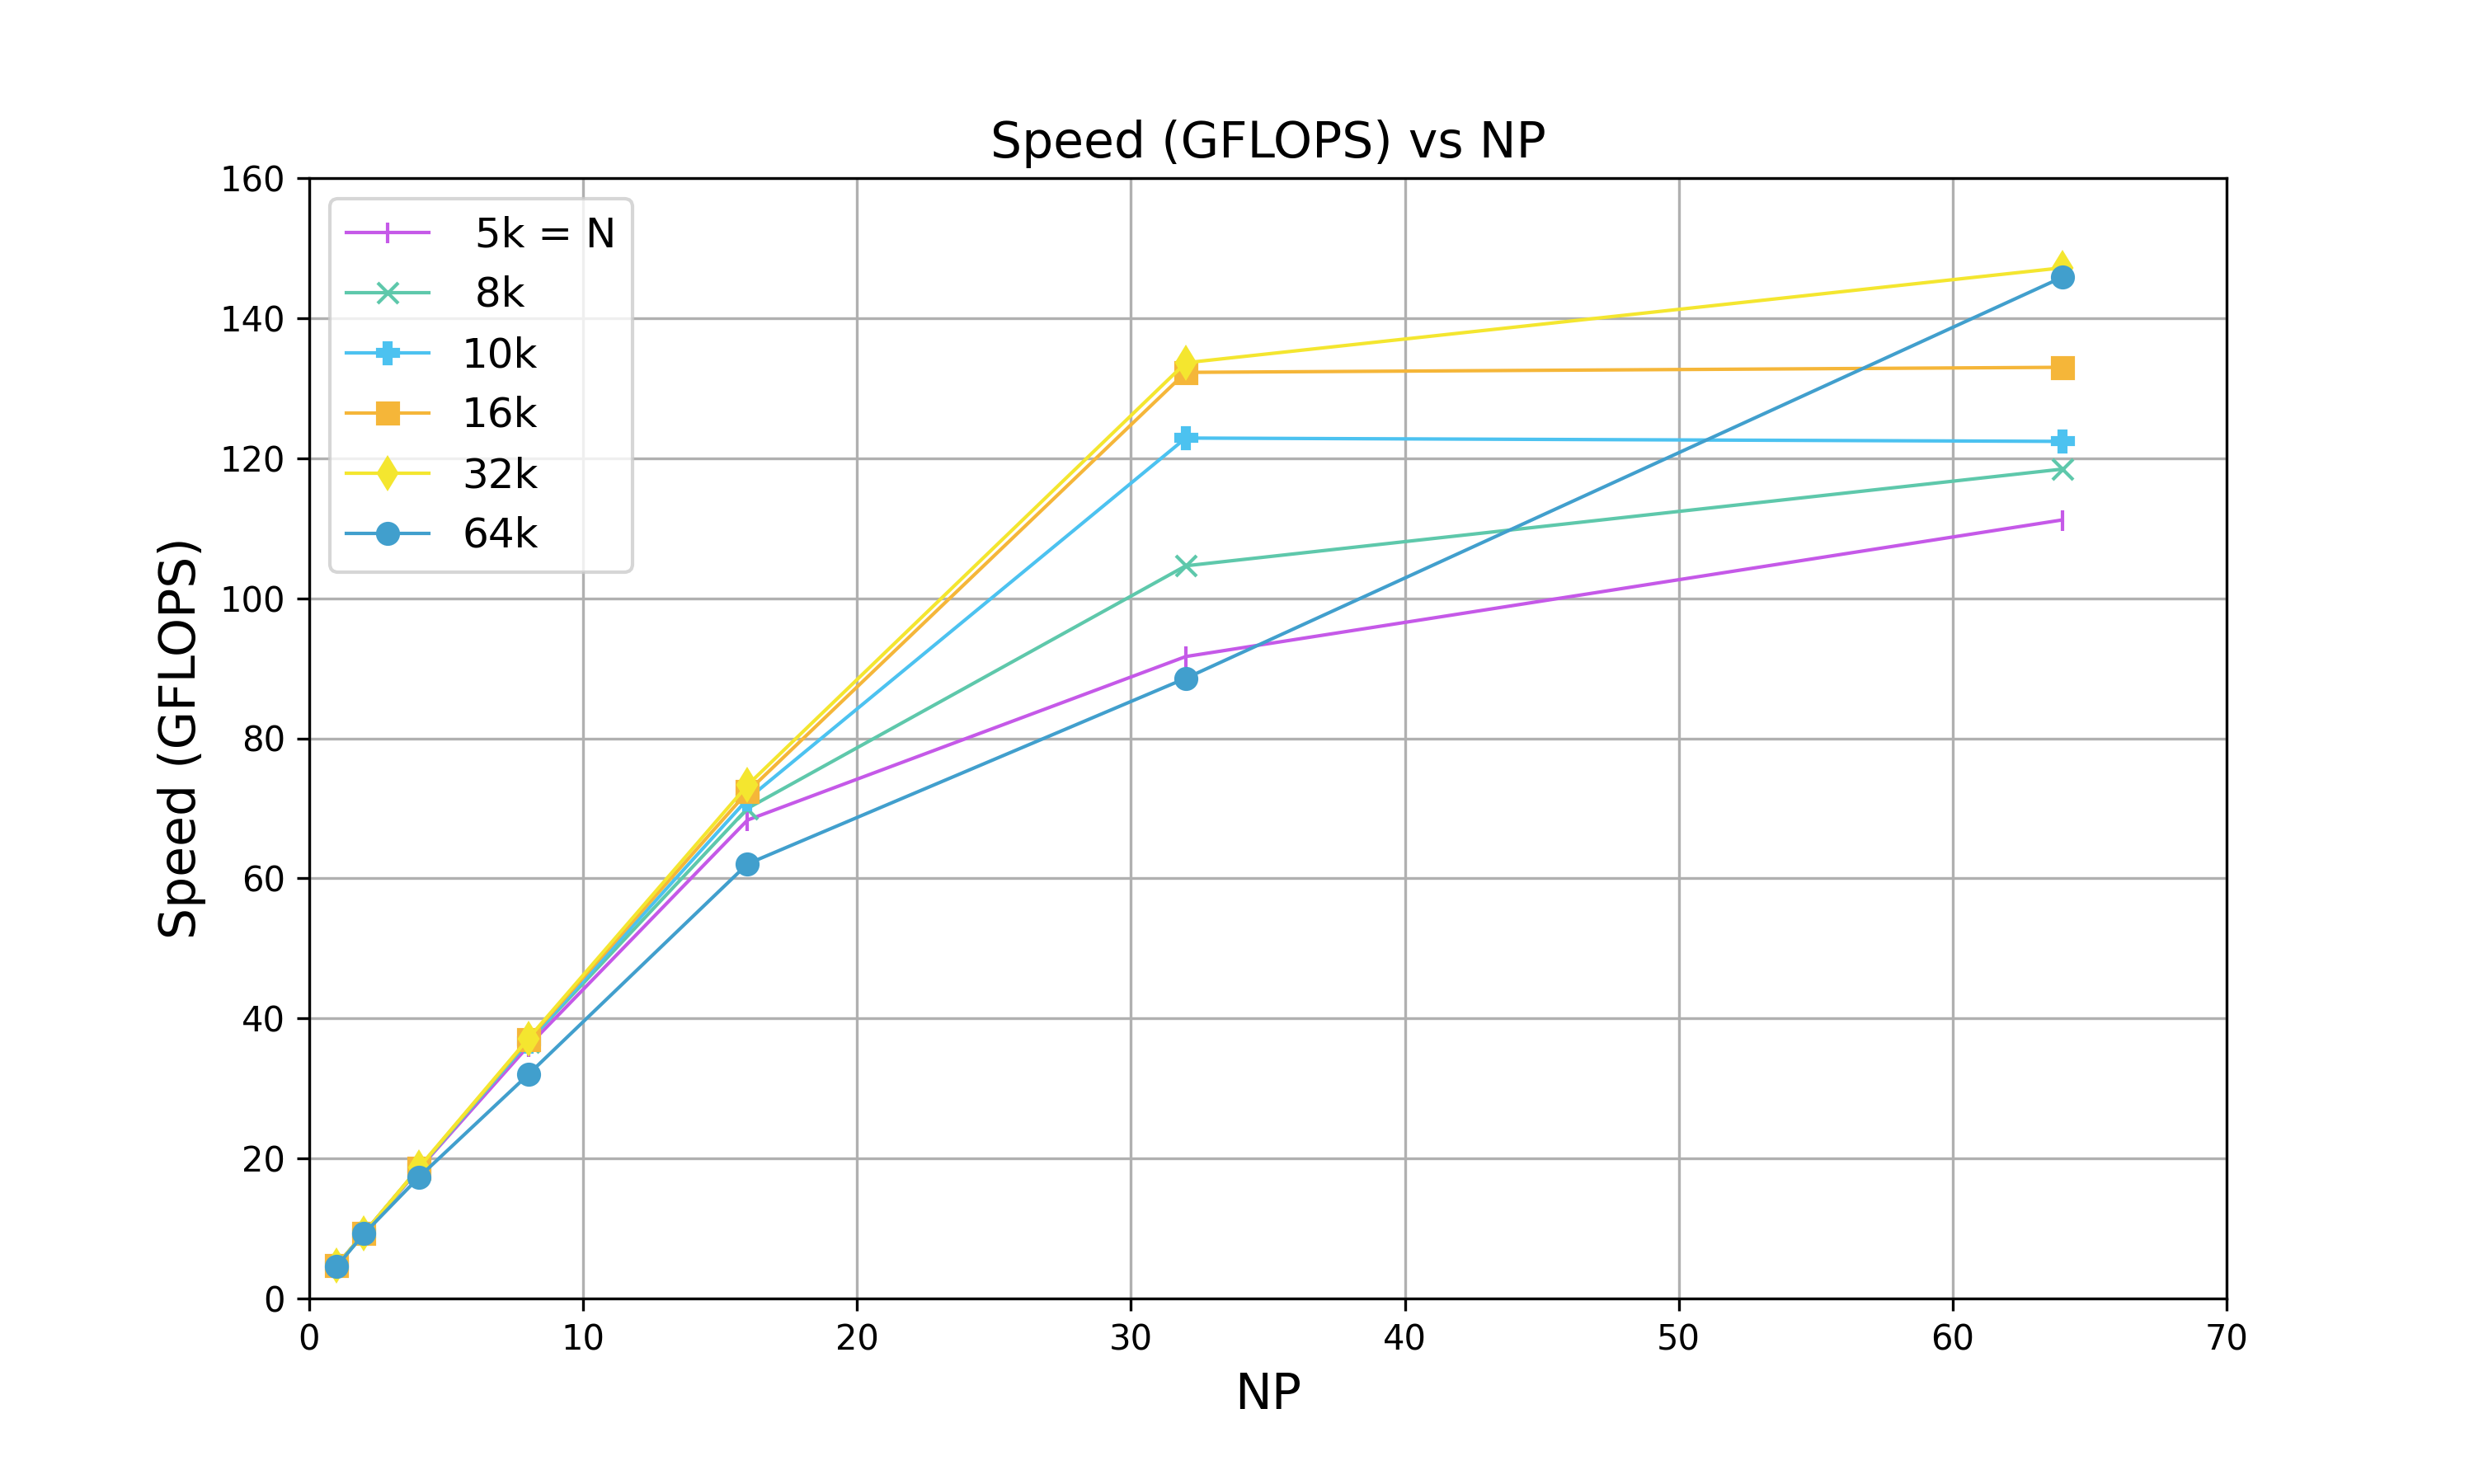
\includegraphics[width =7.5cm]{Images/Speed (GFLOPS) vs NP.png}
    \caption{Speed(GFlops) vs NP}
    \label{fig:my_label}
\end{figure}

\begin{figure}[!ht]
    \centering
    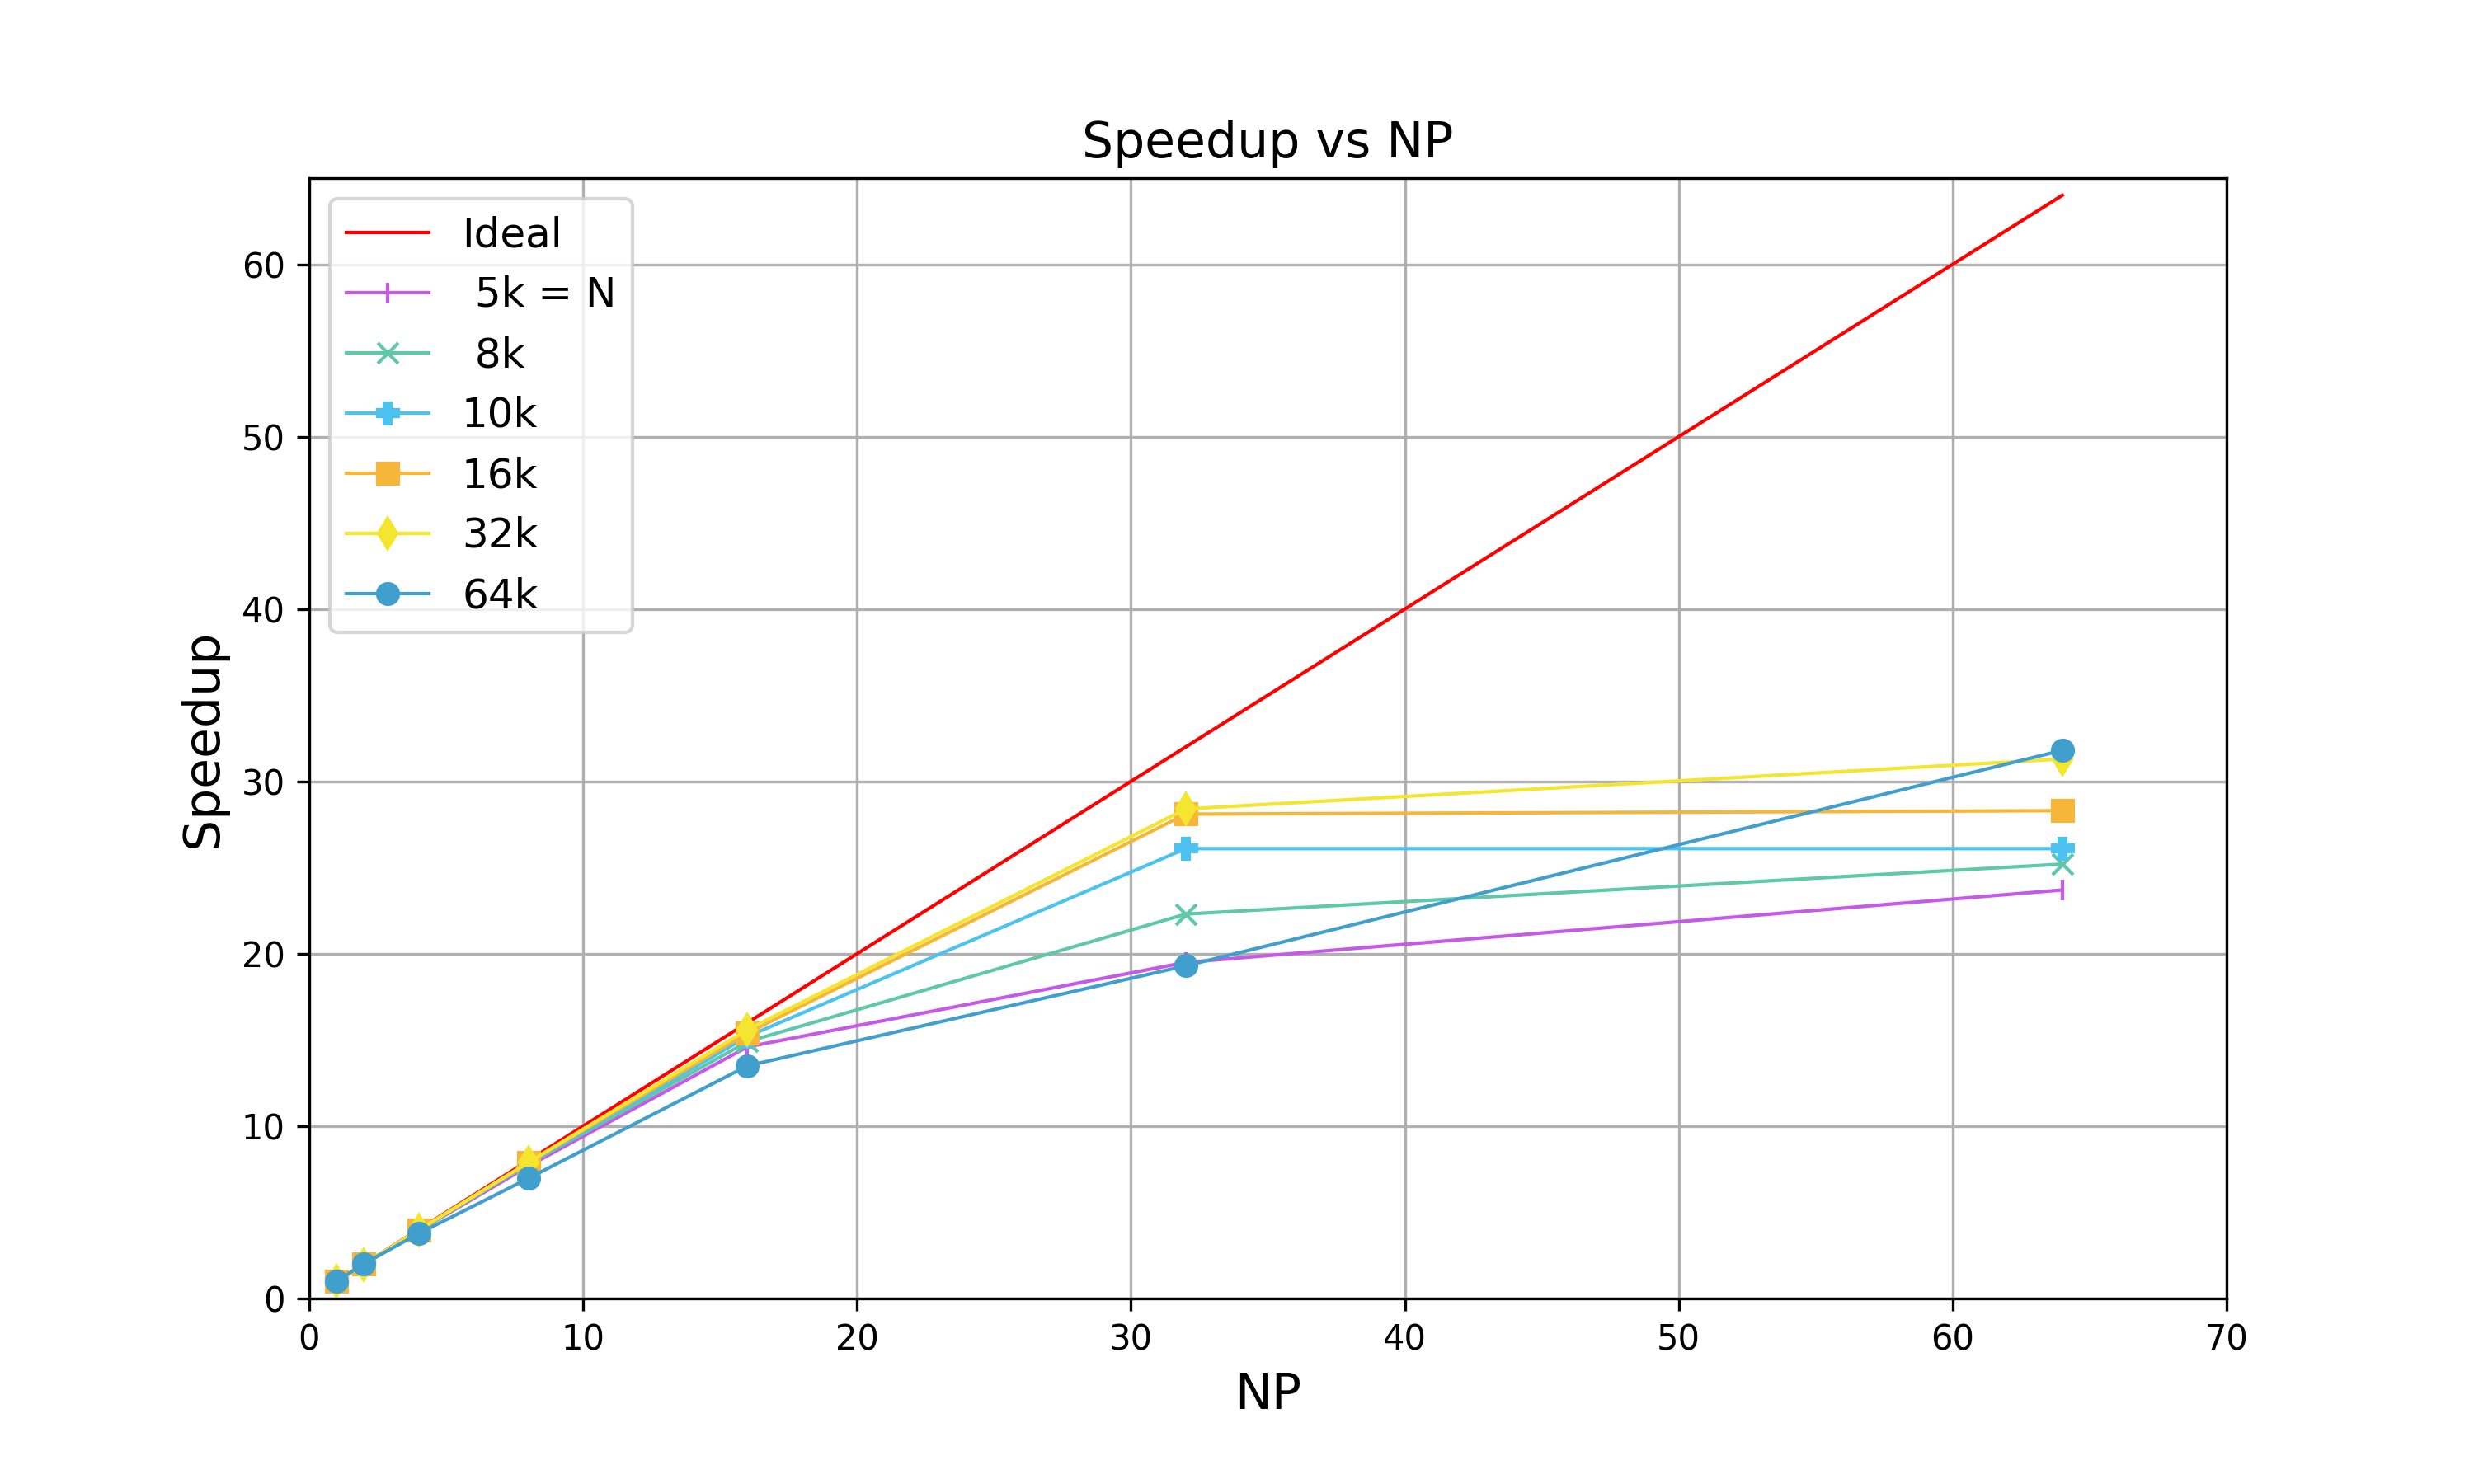
\includegraphics[width =7.5cm]{Images/Speedup vs NP.png}
    \caption{Speedup vs NP}
    \label{fig:my_label}
\end{figure}

\begin{figure}[!ht]
    \centering
    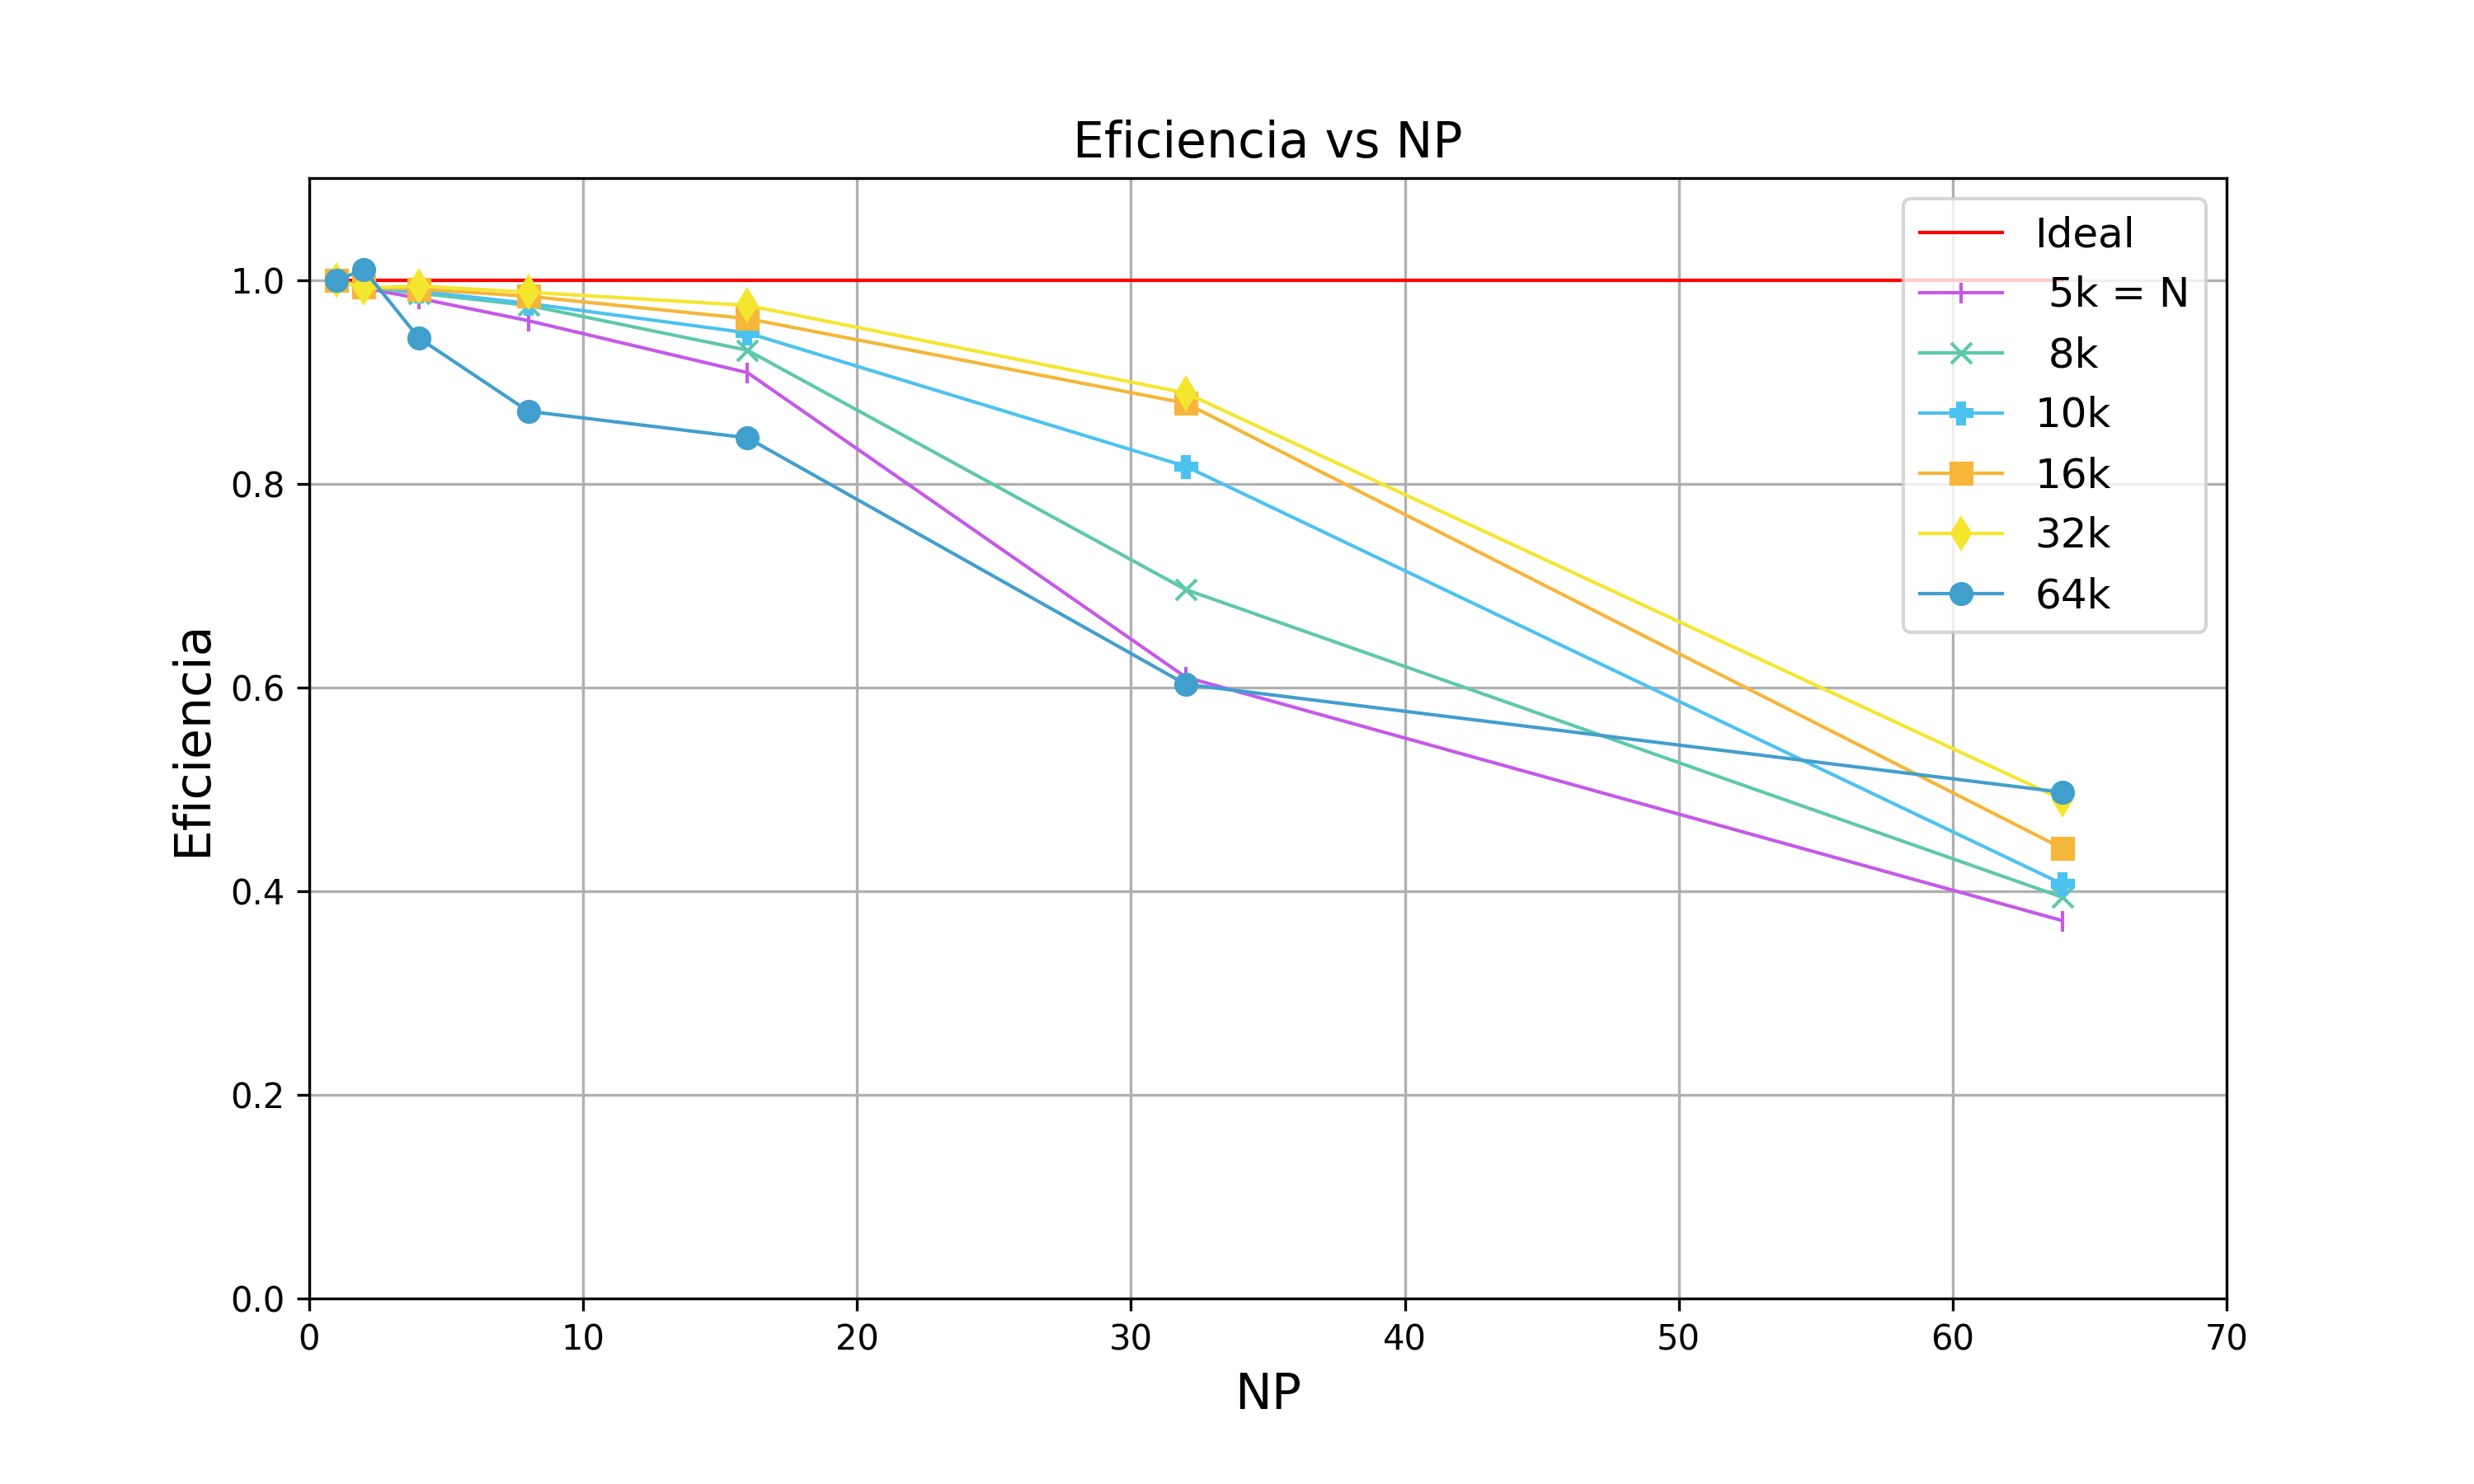
\includegraphics[width =7.5cm]{Images/Eficiencia vs NP.png}
    \caption{Eficiencia vs NP}
    \label{fig:my_label}
\end{figure}

\newpage
\section{ANÁLISIS DE RESULTADOS}
En primer lugar, se analiza el comportamiento que presenta el algoritmo secuencial ($np=1$), por lo que extraemos los datos del tiempo del cálculo de la fuerza. De manera visual, observamos en la figura \ref{fig:complejidad} una complejidad $O(n^2)$ que concuerda con la teórica. Asimismo, los resultados son respaldados con el $r-squared$ el cual indica que la curva experimental se aproxima a la curva teórica. \\

\begin{figure}[!ht]
    \centering
    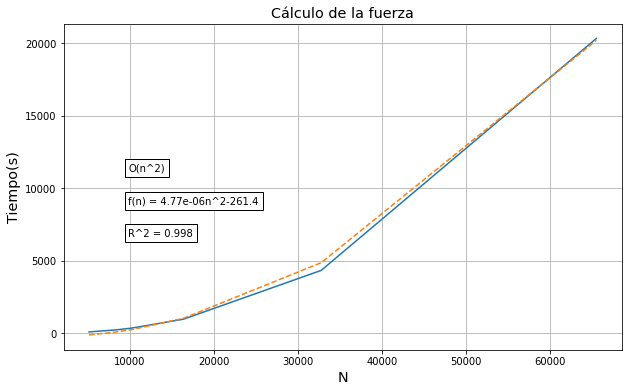
\includegraphics[width =7.5cm]{Images/complejidadv2.png}
    \caption{Complejidad algorítmica}
    \label{fig:complejidad}
\end{figure}

En cuanto, a los tiempos de ejecución que observamos en la figura 3, a medida que se utiliza más procesadores, el problema original se resuelve cada vez más rápido. Este mismo patrón se observa en el tiempo del cálculo de la fuerza, vista en la figura 4. Sin embargo, cuando observamos la figura 5, donde se presenta el tiempo de comunicación entre procesos, al utilizar mayor cantidad de procesos, se aprecia que el tiempo que se emplea es mucho mayor, lo cual es lo esperado. \\

Al observa la gráfica del speedup, en la figura 7, observamos que la curva $N = 32k$ presenta un mejor speedup a comparación de los demás. Asimismo, los resultados se acercan a un speedup lineal cuando utilizamos hasta 16 procesos. Cada vez que vamos aumentando la cantidad de procesos, se van alejando de la curva ideal, presentando una convergencia. \\

Finalmente, cuando observamos la gráfica de eficiencia, en la figura 8, observamos que la curva $N = 32k$ presenta una mejor eficiencia con respecto a los demás. Y, la eficiencia va disminuyendo cada vez que aumentamos la cantidad de procesos, pero, al aumentar el $N$ aumentamos la eficiencia. Es decir, la carga promedio de cada procesador se encuentra más balanceada con respecto a su poder de cómputo.

\section{CONCLUSIÓN}
\begin{itemize}
    \item Según los datos obtenidos, podemos concluir que el algoritmo N-cuerpos optimizado para MPI (Message Passing Interface) que interviene en el cálculo de fuerzas entre partículas nos muestra una gran similitud con lo desarrollado en la parte teórica siguiendo la complejidad de $O(\frac{n^2}{p})$
    \item Creemos que haber realizado una mayor cantidad de experimentos con una mayor cantidad de partículas seguiría respaldado hallado.
    \item En un caso específico, cuando la cantidad de partículas es $N = 32K$ encontramos que su eficiencia es mayor al resto de pruebas con un $N$ diferente.
    \item El tiempo de cálculo de la fuerza nos muestra como disminuye el tiempo de ejecución en relación con el aumento en la cantidad de procesos, ya que este representa el mayor tiempo de cálculo junto con el tiempo de comunicación. Por lo antes expuesto podemos concluir que el algoritmo N-cuerpos paralelizado con MPI que utiliza el proyecto Evolución galáctica es escalable.
\end{itemize}

\section{CÓDIGO FUENTE}
Proyecto Evolución Galáctica, disponible en \href{https://github.com/FabrizioVasquez/CPD_Proyecto_Evolucion_Galactica}{\textt{GitHub}}. 
(https://github.com/FabrizioVasquez/CPD\_Proyecto
\_Evolucion\_Galactica)



\begin{thebibliography}{1}
\bibitem{IEEEhowto:kopka}
Kai Hwang. \emph{Advanced computer architecture}: Parallelism, scalability,programmability. McGraw-Hill, 1993.

\bibitem{IEEEhowto:kopka}
John Gurland and Ram C. Tripathi (1971), \emph{A Simple Approximation for Unbiased Estimation of the Standard Deviation}: The American Statistician 25 (4): 30-32 .

\bibitem{IEEEhowto:kopka}
Measuring Parallel Scaling Performance(2016)[Internet].Disponible en https://www.sharcnet.ca/help/index.php/\\MeasuringParallelScalingPerformanceStrongScaling .

\bibitem{IEEEhowto:kopka}
Introduction to HPC: Scaling tests and profiling for efficient HPC[Internet].Disponible en https://pdc-support.github.io/hpc-intro/10-scaling/ .

\end{thebibliography}

\end{document}
